\documentclass[10pt,a4paper]{article}
\usepackage{graphicx}
\usepackage{amssymb}
\usepackage{fullpage}
\usepackage{amsmath}
\usepackage{url}

\title{Senior Astrophysics 2011 Assignment 2\footnote{Updates can be found at \texttt{https://github.com/goldfish-dave/SeniorAstroAssignment2}}}

\date{}
\author{D. G. Wilcox \\
		309248035}

\begin{document}
\maketitle

\section*{Question 1}
\begin{itemize}
    \item[(a)] A plot of a high, medium and low mass stars.
    Because having all three plots on the same graph makes the features hard to read I've split them into two separate graphs with more suitable scales to the axes.
    \begin{figure}[h!]
        \begin{center}
        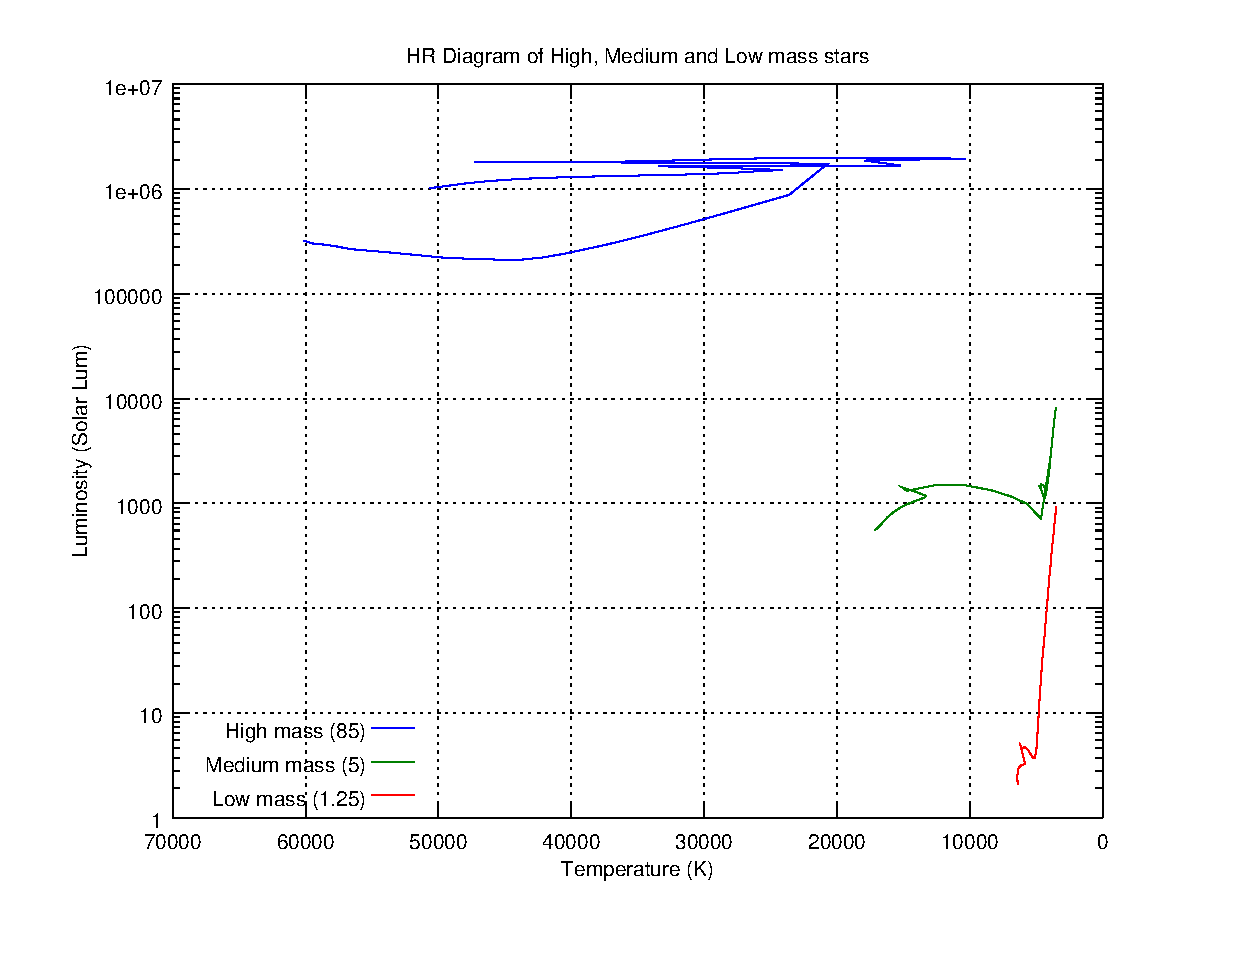
\includegraphics[width=0.8\linewidth]{high-mid-low-HR.eps}
        \caption{High, medium and low masses were taken from table 2, 11 and 18 respectively.}
        \end{center}
    \end{figure}
    \newpage
    \begin{figure}[h!]
        \begin{center}
        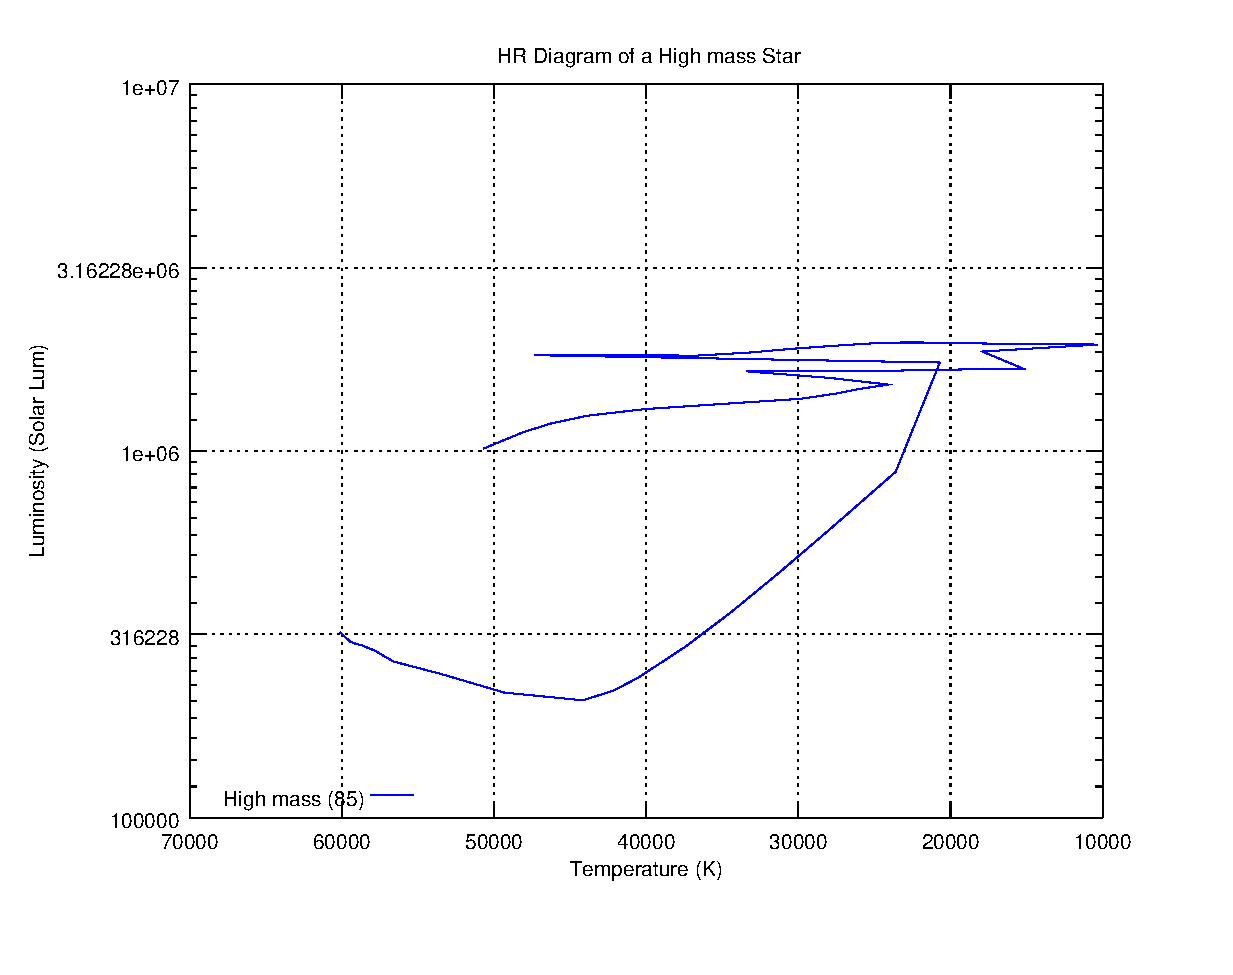
\includegraphics[width=0.8\linewidth]{high-only-HR.eps}
        \caption{A close-up of the high mass star.}
        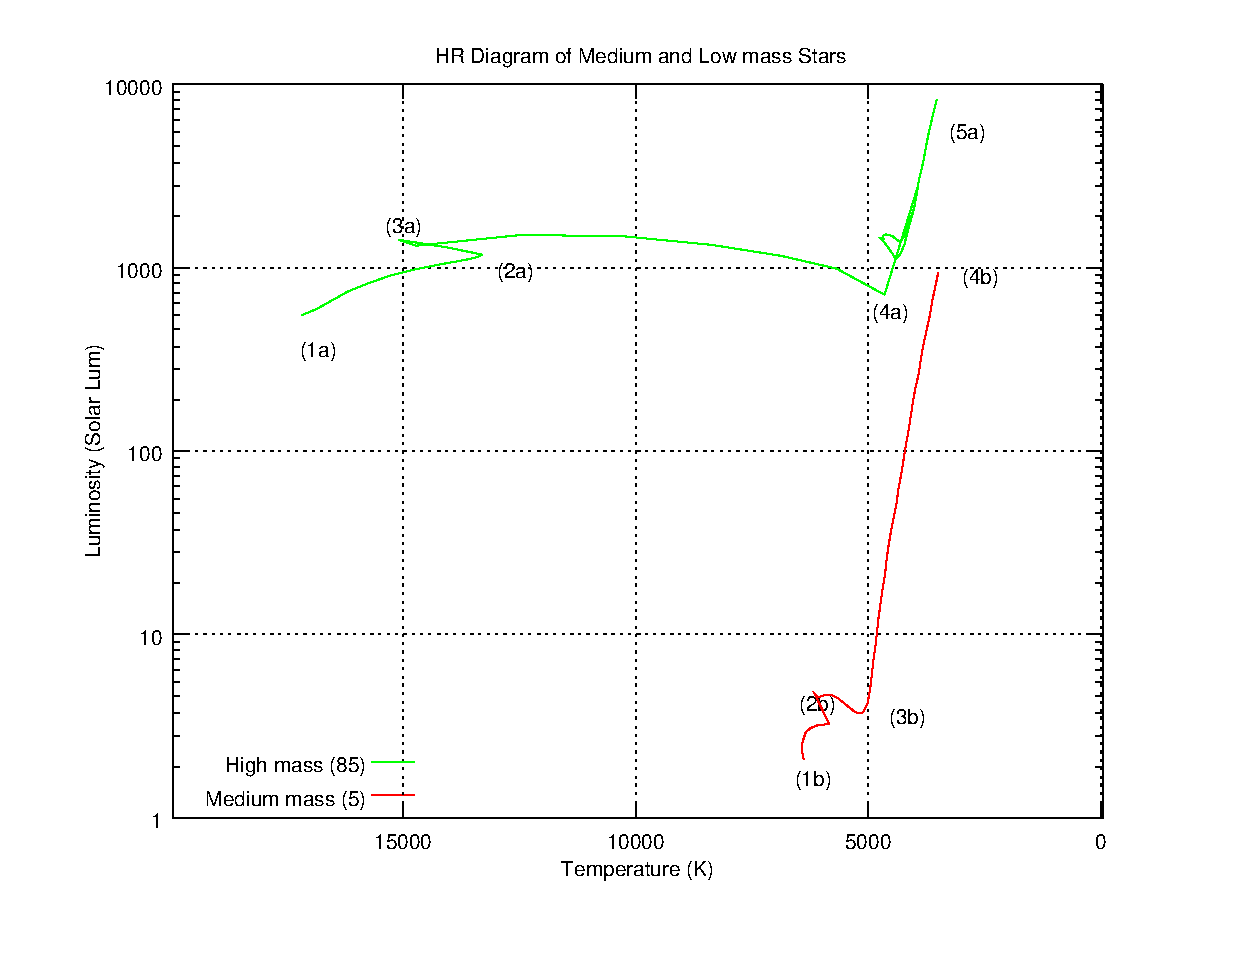
\includegraphics[width=0.8\linewidth]{mid-low-HR.eps}
        \caption{A close-up of the medium and low mass star.}
        \end{center}
    \end{figure}
    \newpage
    \item[(b)]
    \begin{table}[h]
        \begin{tabular}{c|c}
        Location    &   Transition  \\
        \hline \\
        1a  &   Leaves the MS   \\
        2a  &   Subgiant        \\
        3a  &   Red giant       \\
        4a  &   Helium Flash    \\
        5a  &   More flashes after dredge-ups \\
        1b  &   Leaves the MS   \\
        2b  &   Subgiant        \\
        3b  &   Red giant       \\
        4b  &   Helium Flash    \\
        \end{tabular}
    \end{table}
    Unfortunately I've run out of time for this assignment and labeling the high mass star and parts (c),(d) and (e) have not been attempted. Questions 2-4 have been.
    \item[(c)] 
    \item[(d)]
    \item[(e)]
\end{itemize}
\section*{Question 2}
% Reaction Equations
\newcommand{\reactionOne}{$p + p \rightarrow \; ^{2}H + e^{+} + \nu_{e}$}
\newcommand{\reactionTwo}{$^{2}H + p \rightarrow \;^{3}He + \gamma$}
\newcommand{\reactionThree}{$^{3}He + ^{3}He \rightarrow \;^{4}He + 2p$}

% Q-values
\newcommand{\qvalueOne}{$+2.73 \times 10^{5}$}
\newcommand{\qvalueTwo}{$-1.54 \times 10^{7}$}
\newcommand{\qvalueThree}{$-4.24 \times 10^{7}$}

\begin{table}[h]
    \begin{tabular}{c|c|c|c|c}
        \#   &   Reaction            &   LHS Mass   (u)    &   RHS Mass (u)    &   Q-value (MeV) \\
        \hline \\
        1    &   \reactionOne{}      &   2.0145530         &   2.0146486       &   \qvalueOne{}  \\
        2    &   \reactionTwo{}      &   3.0213765         &   3.0160000       &   \qvalueTwo{}  \\
        3    &   \reactionThree{}    &   6.0320000         &   6.0171550       &   \qvalueThree{} \\
    \end{tabular}
\end{table}
Since the entire PP-I chain results in $2(\mbox{Reaction } 1) + 2(\mbox{Reaction } 2) \rightarrow \mbox{Reaction } 3$, if we sub in our values and subtract the left from the right we find that the Q-value for the PP-I chain is $1.22 \times 10^{7}$ MeV, which is in close agreement with the tabulated 12.86 Mev\footnote{\url{http://en.wikipedia.org/wiki/Proton-proton_chain_reaction#The_pp_I_branch}}.
\section*{Question 3}
% Will take unbound to mean not gravitationally interacting.
The remnants of the system post-supernovae will be gravitationally unbound if the following condition holds true:
\begin{equation*}
    F_{G} \leq F_{C}
\end{equation*}
where $F_{G}$ is the attractive force due to gravity and $F_{C}$ is the repulsive force due to the orbital motion. They are described by the following equations:
\begin{align*}
    F_{G} &= G\frac{M_{1}M_{2}}{r^{2}} \\
    F_{C} &= m\omega^{2}r \\
    &\mbox{given:} \\
    \omega^{2} &= G\frac{M_{1}+M_{2}}{r^{3}} \\
\end{align*}
where $G$ is the gravitational constant, $r$ is the separation distance between the two stars and the masses used for Gravity are post-supernovae and the masses used to determine the centripedal motion are pre-supernovae. $m$ is the mass of a test particle.

If we sub in these equations while maintaining our inequality we get the following inequality:
\begin{equation*}
    \Delta m \geq (M_{1}+M_{2})/2
\end{equation*}

\section*{Question 4}
\begin{itemize}
    \item[(a)] If we equate $L=\epsilon \dot M c^{2}$ and $L_{e}=4\pi c G m_{p} M / \sigma_{T}$ we get:
    \begin{align*}
        \dot M &= k M \\
        \mbox{where:}& \\
        k &= \frac{4 \pi G m_{p}}{\epsilon \sigma_{T}c} \\
        \mbox{and }& \\
        m_{p} &= 1.6726 \times 10^{-27} \mbox{ kg} \\
        G &= 6.6730 \times 10^{-11} \mbox{m$^{3}$kg$^{-1}$s$^{-1}$} \\
        c &= 2.9979 \times 10^{8} \mbox { m s$^{-1}$} \\
        \sigma_{T} &= 6.6525 \times 10^{-29} \mbox{ m$^{2}$} \\
        \epsilon &= 0.1 \\
        \mbox{giving:}& \\
        \Rightarrow k &= 7.033 \times 10^{-16} \mbox{ s} \\
    \end{align*}
    \item[(b)] The solution to the differential is:
    \begin{equation*}
        M = M_{0}e^{kt}
    \end{equation*}
    where $M_{0}$ is the initial mass of the black hole and $k$ is from part (a).
    \item[(c)] Using $M_{0} = 100 M_{\odot}$ and $t = 3.154 \times 10^{16}$ seconds we get a black hole mass of $4.27 M_{\odot} \times 10^{11}$. If black holes as massive as $10^{10}M_{\odot}$ already existed at $10^{9}$ yr after the birth of the universe then that would suggest that black holes formed quite early on in the evolution of the universe, assuming our model is correct, as the difference between our calculated value and the measured value is only an order of magnitude (small when dealing with exponentials).
\end{itemize}

\end{document}
